\documentclass[twoside,english]{uiofysmaster}
%\bibliography{references}

\usepackage{array}
\usepackage{booktabs}
\usepackage{float}
\usepackage{scrextend}
\usepackage{amsfonts}
\usepackage{amsmath,amsfonts,amssymb}
\addtokomafont{labelinglabel}{\sffamily}
\usepackage[compat=1.1.0]{tikz-feynman}
\usepackage{tikz}

\usepackage[boxed]{algorithm2e}
\addtokomafont{labelinglabel}{\sffamily}

% Feynman slash
\usepackage{slashed}

% To show code
\usepackage{listings}

% Multicolumns for calculation
\usepackage{multicol}

% Subfigures
\usepackage{subcaption}
\usepackage{sidecap}

\setlength{\heavyrulewidth}{1.5pt}
\setlength{\abovetopsep}{4pt}

\begin{document}

\tableofcontents

\chapter{Supersymmetry at Hadron Colliders}

The Large Hadron Collider (LHC) at CERN is one of the largest and most important particle physics experiments in the world. In this chapter, some of the advantages and challenges of using hadron colliders are discussed, along with some techniques for moving from theory to observable signals. A short description of supersymmetric phenomenology follows, along with current bounds on some supersymmetric particles. Finally, the squark production cross section is calculated to leading order, and next-to-leading order terms are investigated.

\section{Hadron Colliders}

Colliding hadrons makes it possible to reach very high center-of-mass energies, as they allow for the use of circular accelerators. While most linear colliders collide leptons, such as $e^- e^+$, they are not advantageous for circular accelerators because of \textit{synchrotron radiation}. Synchrotron radiation is the radiation of energy from a particle being accelerated. The power radiated by a relativistic charged particle forced to move in circular motion with radius $R$ is given by the Schwinger's formula \cite{Balerna2015}
\begin{align}
P_e = \frac{2}{3} \frac{e^2c }{R^2} \Bigg( \frac{E}{mc^2} \Bigg)^4,
\end{align}
where $E$ is the particle energy, $m$ is the mass and $c$ is the speed of light in vacuum. For light particles, such as leptons, a lot of energy is therefore wasted in circular accelerators. Because the proton mass is much larger than the electron mass, this effect is relatively small, allowing the LHC to operate at energies currently as high as 13 TeV. In this project the data is generated at $8$ TeV. The circular form means the accelerating structures can be reused as many times as one desires, thus putting `no limits' on the energies obtained. There are, of course, limits. At around energies of around $5-7$ TeV per particle, synchrotron radiation becomes an important effect also for protons. The photons emitted from synchrotron radiation hit the walls of the vacuum chamber walls, where they can interact with electrons and cause \textit{electron clouds}. Electron clouds occur when electrons are ejected from the walls of the vacuum chamber and accelerated towards a passing beam bunch. When the electrons reach the center of the chamber, however, the beam bunch has passed, and the now-energetic electrons hit the other side of the chamber, producing more free electrons. This becomes a `cloud' of electrons that can in turn affect the particle beam. 

A challenge more spesific to hadron collisions is the distribution of momentum. Hadrons are made up of valence and sea quarks, which make the kinematics of collisions very difficult to calculate. Valence quarks are the quarks used to classify a hadron, such as $uud$ for the proton and $udd$ for the neutron. In addition to these, hadrons contain a sea of virtual quarks and gluons. The quarks and gluons, the so-called \textit{partons}, distribute the hadron momentum somewhat randomly amongst themselves. Since the distribution of energy and momentum is unknown, so is the momenta of the ingoing parton. To that end the transverse momentum and energy, not to mention the \textit{missing} transverse energy, are important when analysing data from hadron colliders. There is some experimental knowledge of the distribution of longitudinal momentum, however, contained in \textit{parton distribution functions}.

\subsection{Parton Distribution Functions}

Partonic cross sections are calculated for colliding partons, \textit{e.g.} two quarks $q_1 q_2$. The cross section is a function of the center-of-mass energy, $s$, which can be written as a fraction of the center of mass energy of the colliding protons
\begin{align}
s = S x_1 x_2,
\end{align}
where $S$ is the center-of-mass energy of the colliding protons, and $x_i$ is the momentum fraction of the quark $q_i$. The fractions of momenta are then integrated over, using \textit{parton distribution functions} $f(x_i)$, which are specified for the different partons in different hadrons. For example, the fraction $x_u$ for an up-flavour quark in a proton would be much larger than that for a top-flavour quark. Integrating over parton distribution functions yields the total cross section
\begin{align}
\sigma_{q_1q_2} = \int f(x_1) f(x_2) \hat{\sigma}_{q_1q_2}(s) dx_1 dx_2,
\end{align}
where $\hat{\sigma}_{q_1q_2}$ is the partonic cross section. In this project the CTEQ6 parton distribution functions from the LHAPDF Fortran library \cite{PhysRevD.78.013004} are used.

\subsection{Luminosity}

Another important concept is \textit{luminosity}. The instantaneous luminosity $\mathcal{L}$ is a measure on how many collisions happen at a collider per unit time. The integrated luminosity is the luminosity integrated with respect to time, and is here given in inverse femto-barn $\text{fb}^{-1} = 10^{43} \text{ m}^{-2}$. The luminosity of the data can be used to set limits on the size of cross sections, by considering the following relation for a process where a particle $A$ is produced
\begin{align}
n_{A} = \mathcal{L} \sigma_{A} ,
\end{align}
where $\mathcal{L}$ is the integrated luminosity, $\sigma_{A}$ is the cross section for the production of $A$, and $n_A$ is the number of produced particles. Setting $n=1$ for a single produced particle, and using the integrated luminosity for the 8 TeV dataset considered in this project $\mathcal{L} = 20.3 \text{ fb}^{-1}$, the lower limit on cross sections is
\begin{align}
\sigma  = \frac{1}{20.3 \text{ fb}^{-1}} \approx 0.05 \text{ fb}.
\end{align}
Therefore, cross sections below $\sigma \sim \mathcal{O}(10^{-3} \text{ fb}^{-1})$, which correspond to $0.02$ produced particles, will be considered less important in this project.


\section{Phenomenology}

Phenomenology deals with the application of theory to high energy experiments, such as the Large Hadron Collider described in Sec.\ 1.1. This section deals with searches for supersymmetry at hadron colliders, using missing transverse energy and quark jets. Some current bounds on sparticles are discussed as well.

%In order to know what to look for at the LHC it is necessary to consider the phenomenology of supersymmetry. This is done by first revisiting the soft supersymmetry breaking, in order to consider models with more constraints than the 124 parameters of the MSSM. \textit{Hidden sector} (HS) scalar superfields $X$ have very small or no interactions with the MSSM fields. Their couplings are usually supressed by some mass scale so that $\mathcal{L} \sim M^{-1}$. They have an effective (non-renormalizable) interaction  with the scalar superfields of the form
%\begin{align}
%\mathcal{L}_{HS} &= - \frac{1}{M} (\bar{\theta} \bar{\theta}) X \Phi_i \Phi_j \Phi_k.
%\end{align}
%If these sectors develope a vacuum expectation value $\braket{X} = \theta \theta\braket{F_X}$ for the auxilliary field $F$ (auxilliary meaning that it can be removed using the Euler-Lagrange equations),  supersymmetry is broken. The two most commonly known hidden sectors are Planck-scale mediated supersymmetry breaking (PMSB) and Gauge mediated supersymmetry breaking (GMSB), the first of which is obtained by blaming some gravity mechanism for mediating the breaking of SUSY from the hidden sector. The breaking scale is then the Plank scale, $M = M_P = 2.4 \cdot 10^{18}$ GeV. The vev is restricted to $\sqrt{\braket{F}} \sim 10^{10} - 10^{11}$ GeV in order not to reintroduce the hierarchy problem.  The complete soft terms can be shown to be \cite{batzing2017lecture}
%\begin{align*}
%\mathcal{L}_{soft} =& - \frac{\braket{F_X}}{M_P} \Big( \frac{1}{2} f_a \lambda^a \lambda^a + \frac{1}{6} y_{ijk}'A_i A_j A_k + \frac{1}{2} \mu_{ij}' A_i A_j + \frac{\braket{F_X}^*}{M_P^2}  x_{ijk} A_i^* A_j A_k + c.c.\Big)\\
%&- \frac{|\braket{F_X}|^2}{M_P} k_{ij}A_i A_j^*.
%\end{align*}
%By simplifying as much as possible, all soft terms are fixed by just four parameters. This model is called minimal supergravity (mSUGRA) or the constrained minimal supersymmetric Standard Model (CMSSM). The CMSSM parameters are
%\begin{align}
%&m_{1/2} = f \frac{\braket{F_X}}{M_P}, & m_0^2 = k \frac{|\braket{F_X}|}{M_P^2}, 
%&& A_0 = \alpha \frac{\braket{F_X}}{M_P}, &&B_0 = \beta \frac{\braket{F_X}}{M_P},
%\end{align}
%or $m_{1/2}$, $m_0$, $A_0$, $\tan \beta$ and $\text{sgn} \mu$.
%
%The second hidden sector is the aforementioned Gauge mediated supersymmetry breaking. In this case the soft terms come from loop diagrams with \textit{messenger superfields} that get their own mass from coupling to the HS SUSY breaking vev, and have SM interactions. This model is parameterized by 
%\begin{align}
%\Lambda = \frac{\braket{F}}{M_{messenger}} \text{ , } M_{messenger} \text{ , } N_5 \text{ , } \tan \beta,
%\end{align}
%where $M_{messenger}$ is the mass scale and $N_5$ (FYLL INN HER).

\subsection{Searches For Supersymmetry}

Supersymmetry at hadron colliders will likely be in the form of QCD processes, as the colliding particles are quarks and gluons. The traces left in detectors by such processes will be closely related to the conservation of $R$-parity, in that all sparticles are produced in pairs and eventually decay to the LSP. If the LSP is indeed only weakly interacting, this makes it very difficult to detect. An indirect way of detecting it is by looking for \textit{missing transverse energy} $\slashed{E}_T$. The energy is considered solely in the transverse plane, as the longitudinal momentum is difficult to predict in the hadronic case (see the discussion of hadron colliders in Sec.\ 1.1). To look for $\slashed{E}_T$ the \textit{effective mass} is defined as
\begin{align}
M_{eff} &= \sum p_T^{jet} + \slashed{E}_T,
\end{align} 
and used to search for deviations from SM expectations. Here $p_T^{jet}$ is the transverse momentum of \textit{jets}. Jets are collimated bunches of final-state partons and hadrons that appear in hard interactions \footnote{Hard interactions are where the ingoing particles are very energetic}. They can be thought of as energetic partons that undergo showering and the hadronization. Jets are common traces in hadron collision detectors. Because of asymptotic freedom\footnote{The strong coupling constant becomes larger as the distance between partons increases, meaning that partons are \textit{confined} in hadrons.} partons do not remain unbound for long and form the jet hadrons. In supersymmetric processes from hadron collisions the production of jets should also be common, as the LSP is flavour neutral and the color charge of gluinos and squarks must end up in SM particles with color charge. The hadronic jets produced from supersymmetric processes can be complicated, such as the squark-squark production shown in Fig.~\ref{Fig:: susy hadron : decay at ATLAS}. The very large background from SM processes provides another difficulty in searching for supersymmetry. 

\begin{figure}[H]
\centering
\begin{tikzpicture}
\begin{feynman}
\vertex (p1) {\(p\)}; 
\vertex [below right=of p1, blob] (p) {}; 
\vertex [below left=of p] (p2){\(p\)}; 
%----------------------------------
\vertex [right=1.5cm of p] (mid1)
;\vertex [above=0.7cm of mid1] (s1);
\vertex [below =0.7cm of mid1] (s2);
\vertex [right=1.5cm of s1] (q1); 
\vertex [right=1.5cm of s2] (q2) ; 
%---------------------------------
\vertex [below=0.35cm of q1] (midd);
\vertex [right=0.2cm of midd] (r11) {\(\tilde{\chi}_1^0\)}; %W
\vertex [above=0.7cm of r11] (r12) {\(q\)};
%--------------------------------
\vertex [below=0.35cm of q2] (midd2);
\vertex [right=0.2cm of midd2] (k1) {\(\tilde{\chi}_1^0\)};  
\vertex [above=0.7cm of k1] (qq) {\(q\)};
\diagram{
(p1)--(p)--(p2), 
(p) --[scalar, edge label={\(\tilde{q}\)}] (s1), 
(s2) --[scalar, edge label={\(\tilde{q}\)}] (p); 
%----------------------------------
(r11) --[photon, plain] (s1); 
(s1) -- (r12); 
(s2) --[photon, plain] (k1),  
(s2) -- (qq)
};
\end{feynman}
\end{tikzpicture}
\caption{Possible signature of a supersymmetric QCD process, with two quark jets and large missing transverse energy in the final state.}
\label{Fig:: susy hadron : decay at ATLAS}
\end{figure}



Allowing for R-parity violation opens up for more final-state possibilities. The LSP can then decay, and sparticles can be produced one at a time. It is possible to have \textit{massive metastable charged particles} (MMCPs), which are typical for scenarios with a gravitino LSP \cite{batzing2017lecture}.



\subsection{Current Bounds on Sparticles}

Searches and limits are available from the data recorded in 2015 by the ATLAS experiment in $\sqrt{s}=13$~TeV proton-proton collisions at the LHC, with $2.3 \text{ fb}^{-1}$ of analyzed data. The analysis searched for jets and missing transverse energy. Simplified models were assumed, with $R$-parity conservation and the lighest neutralino as the lightest supersymmetric particle. At $95 \%$ confidence level, exclusion limits of the gluino and squark masses are set at $1.51$ TeV and $1.03$ TeV, respectively \cite{aaboud2016search}, assuming a \textit{massless lightest neutralino}. A plot of exclusion limits is shown in Fig.\ \ref{Fig:: susy hadron : ATLAS exclusion limits}. Note that for a massive lightest neutralino the bounds on the gluino and squark masses are significantly reduced, down to $400$ GeV for the squark mass and around $650$ GeV for the gluino mass. Values below these mean that the lightest neutralino is no longer the lightest particle $m_{\tilde{q}} < m_{\tilde{\chi}^0_1}$, $m_{\tilde{g}} < m_{\tilde{\chi}^0_1}$, and sparticles must decay to another particle. In this project squark and gluino masses of $0-4000$ GeV are investigated, as the neutralino is not assumed to be massless.

\begin{figure}[H]
    \centering
    \begin{subfigure}[b]{0.8\textwidth}
        \includegraphics[width=\textwidth]{figures_susy_at_hadron_colliders/ATLAS_excl_mq.png}
        \caption{Squark mass}
    \end{subfigure}
    \begin{subfigure}[b]{0.8\textwidth}
        \includegraphics[width=\textwidth]{figures_susy_at_hadron_colliders/ATLAS_excl_mg.png}
        \caption{Gluino mass}
    \end{subfigure}
    \caption{Exclusion limits from the ATLAS experiment in $\sqrt{s} = 13$ TeV proton-proton collisions. The analysis assumes conservation of $R$-parity and a lightest neutralino LSP. The exclusion limits also assume a massless lightest neutralino. The dashed lines indicate the limit where $m_{\tilde{q}/\tilde{g}} < m_{\tilde{\chi}^0_1}$, so the squarks and gluinos cannot decay to the lightest neutralino above this limit. Figures from \cite{aaboud2016search}.}\label{Fig:: susy hadron : ATLAS exclusion limits}
\end{figure}

%\subsection{Precision Observables}

%We can also measure SUSY by considering its impact on very precisey measured SM processes, such as electroweak precision observables, the $(g-2)_{\mu}$ value, the flavour changing neutral current (FCNC) process $b \rightarrow s \gamma$ and the (rare) FCNC process $B_s \rightarrow \mu \mu$.
%
%The electroweak precision observables include $M_W$, $M_Z$, $\Gamma_W$, $\Gamma_Z$, $m_t$ and $\sin \theta_W$, the higgs mass $m_h$ and its properties. Since the Higgs has been measured, we can now do very precise measurements of these quantities, and find that they are very consistent with SM predictions.
%
%The anomalous magnetic moment of the muon, $(g - 2)_{\mu}$, has been measured to extraordinary precision at BNL to be
%\begin{align*}
%g_{\mu} = 2.00116592089(63),
%\end{align*}
%where the digits in parenthesis indicate the uncertainty on the last digits. At tree level we have $\mu \rightarrow \mu \gamma$. Loop corrections to this diagram give $a_{\mu} = (g -2)_{\mu}$. The difference between the SM deviation and the experimentally measured deviation is
%\begin{align*}
%\delta_{a_{\mu}} \equiv a_{\mu}^{exp} - a_{\mu}^{SM}= (25.9 \pm 8.1) \cdot 10^{-10},
%\end{align*}
%which is $3.2 \sigma$ away from zero. This is one of the clearest discrepancies that exist between measurement and the SM.


\section{Squark-Squark Cross Section}
In this project the relevant QCD process will be the production of squark pairs in quark-quark collisions,
\begin{align}
q_i q_j \rightarrow \tilde{q}_i \tilde{q}_j,
\end{align}
where $i,j$ are the 4 light quark flavours $u, d, s, c$. Feynman diagrams for tree-level contributions are found in Fig.\ \ref{Fig:: susy hadron : Feynman qq}. For equal flavour quarks the $t$- and $u$-channel contribute, while only the $t$-channel contributes for different flavours. 

\begin{figure}
\centering
\begin{tikzpicture}
\begin{feynman}
\vertex (p1) {\(q_i\)}; \vertex [right= of p1] (s1); \vertex [right= of s1] (q1){\(\tilde{q}_i\)}; \vertex [below=of p1] (p2) {\(q_j\)}; \vertex [right=of p2] (s2) ; \vertex [right= of s2] (q2) {\(\tilde{q}_j\)} ;
\diagram{
(p1) --[fermion, momentum=\(k_1\)] (s1) -- [scalar, momentum=\(p_1\)] (q1), (s1)-- [gluon] (s2) -- (s1), (p2) --[fermion, momentum=\(k_2\)] (s2) --[scalar, momentum=\(p_2\)] (q2)
};
\end{feynman}
\end{tikzpicture}
\begin{tikzpicture}
\begin{feynman}
\vertex (p1) {\(q_i\)}; \vertex [right= of p1] (s1); \vertex [right= of s1] (q1){\(\tilde{q}_i\)}; \vertex [below=of p1] (p2) {\(q_j\)}; \vertex [right=of p2] (s2) ; \vertex [right= of s2] (q2) {\(\tilde{q}_j\)} ;
\diagram{
(p1) --[fermion] (s1) -- [scalar] (q2), (s1)-- [gluon] (s2) -- (s1), (p2) --[fermion] (s2) --[scalar] (q1)
};
\end{feynman}
\end{tikzpicture}
\caption{Feynman diagrams for squark pair production in quark quark collisions, both $t$ and $u$ diagram. Note that the u-channel (right diagram) is only possible for $i=j$.}
\label{Fig:: susy hadron : Feynman qq}
\end{figure}


%\subsection{Feynman Diagrams}

\subsection{Leading Order Cross Section}

In this section the partonic cross section for squark pair-production is calculated to leading order. The exchanged gluino momentum is denoted $p$ in the calculations, and defined as $p= k_2-p_2 $ for the $t$-channel and $p=k_2-p_1$ for the $u$-channel. The following set of kinematical invariants are used
\begin{align*}
s &= (k_1 + k_2)^2 = 2 k_1 \cdot k_2, &t_1 = (k_2-p_2)^2 - m_{\tilde{q}}^2, &&t_g = (k_2-p_2)^2 - m_{\tilde{g}}^2,\\
t &= (k_2-p_2)^2 = m_{\tilde{q}}^2 - 2 (k_2 \cdot p_2), &u_1 = (k_1-p_2)^2 - m_{\tilde{q}}^2, &&u_g = (k_1-p_2)^2 - m_{\tilde{g}}^2,\\
u &= (k_1 - p_2)^2 = m_{\tilde{q}}^2 - 2 (k_1 \cdot p_2),
\end{align*}
where the Mandelstam variables are related by $t + u+ s = p_1^2 + p_2^2$. The expressions for the different chiralitites are considered later, until then the chiral projection operators in the matrix element are denoted as $P$ and $P'$. The Feynman gauge is used, and the $n_f = 5$ light flavour quarks are treated as massless. 

\subsubsection{Pure $t$-channel}

The matrix element for the pure $t$-channel becomes (reading direction is from $q_j$ to $q_i$)
\begin{align*}
i \mathcal{M}_t &= \bar{v} (k_1) \Big( -i \sqrt{2} g P (t_a)^{ij}\Big) \times \delta^{ab} \frac{i}{\slashed{p} - m_{\tilde{g}}} \times \Big( -i \sqrt{2} gP'(t_b)^{lk} \Big) \times u(k_2)\\
&= - (t_a)^{ij}(t^a)^{lk} \times \frac{i 2 g^2}{t_g^2} \times  \bar{v} (k_1)  P (\slashed{p} + m_{\tilde{g}}) P' u(k_2) ,
\end{align*}
where the color factor has been factored out. The matrix element squared is then
\begin{align*}
|\mathcal{M}_t|^2 &=  (t_a)^{ij} (t^a)^{lk} (t_b)_{ij} (t^b)_{lk} \times \frac{4 g^4}{t_g^2}
\big( \bar{v} (k_1)  P (\slashed{p} + m_{\tilde{g}}) P' u(k_2) \big)
\big( \bar{u} (k_2)  P (\slashed{p} + m_{\tilde{g}}) P' v(k_1) \big).
\end{align*}
To sum over colors, the following relation is used \cite{ellis2003qcd}
\begin{align}
\sum_a (t^a)_{ij} (t_a)_{lk} = \frac{1}{2} (\delta_{ik} \delta_{lj} - \frac{1}{N} \delta_{ij} \delta_{lk}),
\end{align}
which gives for the color factor
\begin{align*}
(t^a)^{ij}(t_a)^{kl}(t^b)_{ij}(t_b)_{kl} &= \frac{1}{4} 
\big(\delta_{ik} \delta_{lj} - \frac{1}{N} \delta_{ij} \delta_{lk} \big)
\big(\delta^{ik} \delta^{lj} - \frac{1}{N} \delta^{ij} \delta^{lk} \big) = \frac{1}{4} (N^2 - 1) = \frac{1}{2}NC_F,
\end{align*}
where $C_F = (N^2 - 1)/(2N)$. Averaging over spin
\begin{align*}
\sum |\mathcal{M}_t|^2 &= \frac{1}{2} NC_F \times \frac{4 g^4}{t_g^2} \text{tr} \big[ 
\slashed{k}_1 P (\slashed{p} + m_{\tilde{g}}) P' \slashed{k}_2 P (\slashed{p} + m_{\tilde{g}}) P' \big].
\end{align*}
As previously mentioned, the quark masses are set to zero. The final state squarks can have equal or different chiralities, both of which contribute to the total cross section.

\subsubsection{Different chiralities $P=P_{R/L}$, $P'=P_{L/R}$}
In the case of different chiralities the trace becomes
\begin{align*}
\text{tr} \big[ 
\slashed{k}_1 P_{R/L} (\slashed{p} + m_{\tilde{g}}) P_{L/R} \slashed{k}_2 P_{R/L} (\slashed{p} + m_{\tilde{g}}) P_{L/R} \big]
&= 2 \big(
2 (p \cdot k_2) (k_1 \cdot p) - p^2 (k_1 \cdot k_2)\big)\\
& = (t-m_{\tilde{q}}^2)s + (t-m_{\tilde{q}}^2)(u-m_{\tilde{q}}^2)-  ts\\
&=  t_1u_1 -m_{\tilde{q}}^2s.
\end{align*}
For same flavour ingoing quarks $qq$, there is one possibility for different chiralities $\tilde{q}_R\tilde{q}_L$. For different flavours $q'q$ there are two possibilities; $ \tilde{q}_R \tilde{q}'_L$ and $\tilde{q}_L \tilde{q}'_R$.  


\subsubsection{Equal chiralities $P=P_{R/L}$, $P'=P_{R/L}$}
In the case of equal chiralities the trace becomes
\begin{align*}
\text{tr} \big[ 
\slashed{k}_1 P_{R/L} (\slashed{p} + m_{\tilde{g}}) P_{R/L} \slashed{k}_2 P_{R/L} (\slashed{p} + m_{\tilde{g}}) P_{R/L} \big]&= 2  m_{\tilde{g}}^2 (k_1 \cdot k_2)= m_{\tilde{g}}^2 s,
\end{align*}
where $P_{R/L}P_{R/L} = P_{R/L}$, $(\gamma^5)^2 = 1$ and $\text{tr}[\gamma^5 \gamma^{\mu} \gamma^{\nu}]=0$. For equal flavour quarks $qq$ there are now two possibilities for equal chiralities: $\tilde{q}_R \tilde{q}_R$ and $ \tilde{q}_L \tilde{q}_L$. For different flavour quarks $qq'$ there are two possibilities for equal chiralities: $ \tilde{q}_L \tilde{q}'_L$ and $\tilde{q}_R \tilde{q}_R'$. 

Note that the contribution from $\tilde{q}_R \tilde{q}_R$ is identical to $\tilde{q}_L \tilde{q}_L$ in QCD processes. If no electroweak corrections are included in the higher order term, the NLO cross section should also be identical as a function of $m_{\tilde{q}}$, because only the electroweak interaction couples to right- and left-handed states differently. 

\subsubsection{Sum over Chiralities}

For incoming quarks $q_iq_j$ the sum over chiralities  yields
\begin{align*}
\sum |\mathcal{M}_t|^2 =  NC_F  \times\frac{4 g^4}{t_g^2} \Big[\delta_{ij} \big(\frac{1}{2}(t_1u_1 -sm_{\tilde{q}}^2)+  sm_{\tilde{g}}^2 \big) + (1-\delta_{ij})\big(t_1u_1 -s(m_{\tilde{q}}^2- m_{\tilde{g}}^2) \big)\Big].
\end{align*}

\subsubsection{Pure $u$-channel}

The expression for the $u$-channel diagram is identical to the $t$-channel, but for the exchange $t_g^2 \rightarrow u_g^2$. The $u$-channel only contributes in the case where $i =j$, so the matrix element is
\begin{align*}
\sum |\mathcal{M}_u|^2 &= \delta_{ij} NC_F \frac{4g^4}{u_g^2} \Big[ \frac{1}{2}(t_1u_1-sm_{\tilde{q}}^2) + sm_{\tilde{g}}^2 \Big]. 
\end{align*}


\subsubsection{Cross term}
The $ut$ cross term has the matrix element $\mathcal{M}_{tu}+ \mathcal{M}_{ut}$, where $\mathcal{M}_{tu}$ is given by
\begin{align*}
i \mathcal{M}_{tu} &= (t^a)^{ij}(t_a)^{kl}(t^b)_{ik}(t_b)_{jl} \frac{-i 2 g^2}{t_g}\big( \bar{v} (k_1)  P (\slashed{p} + m_{\tilde{g}}) P'u(k_2) \big)  \frac{i 2 g^2}{u_g} \big( \bar{u} (k_2)  P (\slashed{p} + m_{\tilde{g}}) P' v(k_1) \big)\\
\end{align*}
The color factor is
\begin{align*}
\sum_{a,b}(t^a)^{ij}(t_a)^{kl}(t^b)_{ik}(t_b)_{jl} 
 &= - \frac{1}{2}C_F.
\end{align*}
Average over spins
\begin{align*}
\sum \mathcal{M}_{tu} &= - \frac{1}{2}C_F \times \text{tr}\Bigg[ \frac{4 g^4}{u_gt_g}\big( \slashed{k}_1   P (\slashed{k}_2 - \slashed{p}_2 + m_{\tilde{g}}) P'\slashed{k}_2  P (\slashed{k}_2 -\slashed{p}_1 + m_{\tilde{g}}) P' \big) \Bigg].
\end{align*}
Summing over equal and different chiralities gives
\begin{align*}
\sum  \mathcal{M}_{tu} 
  &= - \frac{1}{2}C_F  \frac{4 g^4}{u_gt_g} \big(
  -   t_1 u_1 + m_{\tilde{q}}^2 s 
+  m_{\tilde{g}}^2 s
  \big)\\
\end{align*}
The other term --  $\mathcal{M}_{ut}$ -- is similar, but yields a slightly different combination
\begin{align*}
\sum i \mathcal{M}_{ut} 
  &= - \frac{1}{2}C_F  \frac{4 g^4}{u_gt_g} \big(
u_1t_1- m_{\tilde{q}}^2s + m_{\tilde{g}}^2s
  \big).
\end{align*}
Adding the cross terms then gives 
\begin{align*}
\sum |\mathcal{M}_{ut+tu}| &= - \frac{1}{2}C_F \delta_{ij}  \frac{4 g^4}{u_gt_g} \big(2 m_{\tilde{g}}^2s   \big).
\end{align*}


\subsubsection{Matrix Elements}

The matrix elements can be divided into contributions from $\tilde{q}_{iR} \tilde{q}_{iR}$, $\tilde{q}_{iR} \tilde{q}_{iL}$, $\tilde{q}_{iR} \tilde{q}_{jR}$ and $\tilde{q}_{iR} \tilde{q}_{jL}$, and equivalently for $R \leftrightarrow L$. These are
\begin{align}
&\tilde{q}_{iR} \tilde{q}_{iR}, \tilde{q}_{iL} \tilde{q}_{iL}: && \sum |\mathcal{M}|_{iRiR} = 4g^4 s m_{\tilde{g}}^2 \Big[ \frac{1}{2} NC_F\Big( \frac{1}{t_g^2} + \frac{1}{u_g^2} \Big) - C_F \frac{1}{t_gu_g} \Big],\\
&\tilde{q}_{iR} \tilde{q}_{iL}: &&\sum |\mathcal{M}|_{iRiL}=  4 g^4 (u_1t_1 - sm_{\tilde{q}}^2) \Big[ \frac{1}{2}NC_F \Big( \frac{1}{t_g^2} + \frac{1}{u_g^2} \Big) \Big],\\
& \tilde{q}_{iR} \tilde{q}_{jR}, \tilde{q}_{iL} \tilde{q}_{jL}: && \sum |\mathcal{M}|_{iRjR} = 4 g^4 sm_{\tilde{g}}^2 \Big[\frac{1}{2} NC_F \frac{1}{t_g^2}  \Big],\\
& \tilde{q}_{iR} \tilde{q}_{jL}, \tilde{q}_{iL} \tilde{q}_{jR}: && \sum |\mathcal{M}|_{iRjL} = 4 g^4 (t_1u_1 - sm_{\tilde{q}}^2) \Big[\frac{1}{2} NC_F \frac{1}{t_g^2}  \Big],\\
\end{align}

Summing over the terms from different chirality combinations gives  for the total sum over matrix element squared 
\begin{align}
\sum |\mathcal{M}|^2 = \delta_{ij} & \Bigg[2 g^4NC_F(u_1t_1-sm_{\tilde{q}}^2) \Big( \frac{1}{t_g^2} + \frac{1}{u_g^2} \Big) \nonumber \\& + 4 g^4 sm_{\tilde{g}}^2 \Big( NC_F \Big(\frac{1}{t_g^2} + \frac{1}{u_g^2}\Big) -2C_F\frac{1}{u_gt_g} \Big) \Bigg] \nonumber \\
+& (1-\delta_{ij})\Bigg[4g^4NC_F  \frac{u_1t_1-s(m_{\tilde{g}}^2-m_{\tilde{g}}^2)}{t_g^2} \Bigg].
\end{align}



\subsection*{Partonic Cross Section}

The $SU(3)$ color factors are given by $N=3$, and therefore $C_F = 4/3$. To find the total, lowest order partonic cross section an $n$-dimensional phase space integral is performed, and spin and color averaging are taken into account \cite{beenakker1997squark}. The lowest order double-differential distributions are then given by
\begin{align}
s^2 \frac{d^2 \sigma^B}{dt du} =&  K_{ij} \frac{\pi S_{\varepsilon}}{\Gamma(1 - \varepsilon)} \Bigg[ \frac{(t-p_2^2)(u-p_2^2) - p_2^2s}{\mu^2s} \Bigg]^{- \varepsilon} \Theta ([t-p_2^2][u- p_2^2]-p_2^2s) \nonumber \\
& \times \Theta (s -4m^2) \delta (s+t+u-p_1^2 -p_2^2) \sum |\mathcal{M}_B|^2,
\end{align} 
where the averaging over initial state colours and spins is given by the factor $K_{ij}$, which for squark and antisquark prodution is \cite{beenakker1997squark}
\begin{align}
K_{qq} = K_{\bar{q}q} = \frac{1}{4 N^2}.
\end{align}
Integration over the remaining parameters gives for squark production $q_iq_j \rightarrow \tilde{q}_i \tilde{q}_j$ \cite{beenakker1997squark}
\begin{align}\label{Eq:: susy hadron : Born term sigma}
\hat{\sigma}^B =& \frac{\pi \alpha_s^2}{s} \Bigg[\beta_{\tilde{q}} \Big(-\frac{4}{9} - \frac{4m_-^4}{9(m_{\tilde{g}}^2s+m_-^4)} \Big) + \Big(-\frac{4}{9}- \frac{8m_-^2}{9s} \Big) L_1 \Bigg] \nonumber \\
&+ \delta_{ij} \frac{\pi \alpha_s^2}{s} \Bigg[ \frac{8m_{\tilde{g}}^2}{27(s+2m_-^2)} L_1 \Bigg],
\end{align}
where
\begin{align*}
&L_1 = \ln \Big( \frac{s+2m_-^2-s \beta_{\tilde{q}}}{s+ 2m_-^2+s \beta_{\tilde{q}}} \Big), &\beta_{\tilde{q}} = \sqrt{1-\frac{4m_{\tilde{q}}^2}{s}}, &&m_-^2 = m_{\tilde{g}}^2 - m_{\tilde{q}}^2, &&\alpha_s = \frac{g_s^2}{4 \pi}.
\end{align*}
The cross section for antisquark pair production is similar.

\section{Next-to-leading Order Corrections}

The next-to-leading order (NLO) terms contain virtual corrections to the Born level, or tree-level, Feynman diagrams. By allowing more complicated Feynman diagrams, virtual particles can appear in the process. These never make it to the final state and become real particles, but are instead absorbed by the process. Since they are never real, or on-shell, they can have any momentum and mass. Thus, it is necessary to integrate over all possible momenta, which leads to divergences and infinities. 

There are three main categories of divergences, namely ultraviolet, infrared and collinear. Ultraviolet divergences appear when the integral is over an energy without upper bounds. When the opposite problem occurs, that low momentum gives infinities, this is called an infrared divergence. Collinear divergences are also called mass singularities, and stem from exactly that --- masses going to zero, where infinities can appear from splitting at zero angle.

\begin{figure}
    \centering
    \begin{subfigure}[b]{0.8\textwidth}
        \begin{tikzpicture}
\begin{feynman}
\vertex (p1); \vertex [right= 1cm of p1, blob] (s1) {}; \vertex [right=1.4cm of s1] (q1);
\diagram{
(p1) -- (s1) , (p1) -- [gluon]  (s1), (q1) -- (s1) -- [gluon] (q1)
};

\hspace{3.3 cm}
\node {=};
\hspace{0.3 cm}

\vertex (p2); \vertex [right= 1cm of p2] (s2); \vertex [right=1cm of s2] (q2); \vertex [right = 1cm of q2] (r2);
\diagram{
(p2) -- (s2) -- [gluon, half right] (q2), (p2) -- [gluon]  (s2),(q2)-- [gluon, half right] (s2) -- [half left] (q2), (q2) -- [gluon] (r2) -- (q2)
};

\hspace{3.3 cm}
\node {+};
\hspace{0.3 cm}

\diagram{
(p2) -- (s2) -- [fermion, half right] (q2), (p2) -- [gluon]  (s2),(q2)-- [scalar, half right] (s2), (q2) -- [gluon] (r2) -- (q2)
};
\hspace{3.3 cm}
\node {+};
\hspace{0.3 cm}
\diagram{
(p2) -- (s2),(q2) -- [fermion, half right] (s2), (p2) -- [gluon]  (s2),(s2)-- [scalar, half right] (q2), (q2) -- [gluon] (r2) -- (q2)
};
\end{feynman}
\end{tikzpicture}
        \caption{Gluino self-energy.}
        \label{fig:gull}
    \end{subfigure}
    ~ %add desired spacing between images, e. g. ~, \quad, \qquad, \hfill etc. 
      %(or a blank line to force the subfigure onto a new line)
    \begin{subfigure}[b]{0.8\textwidth}
        \begin{tikzpicture}
\begin{feynman}
\vertex (p1); \vertex [right = 1 cm of p1, blob] (s1) {}; \vertex [above right= 1 cm of s1] (q1); \vertex [below right = 1cm of s1] (r1);
\diagram{
(p1) -- [fermion] (s1), (s1) -- [gluon] (r1) -- (s1), (s1) -- [scalar] (q1)
};

\hspace{2.5 cm}
\node {=};
\hspace{0.3 cm}

\vertex (p2); \vertex [right = 1 cm of p2] (s2); \vertex at (2.0,0.4) (q2); \vertex at (2.5, 0.7) (q22); \vertex at (2.0,- 0.4) (r2); \vertex at (2.5, -0.7) (r22);
\diagram{
(p2) -- [fermion] (s2); (s2) -- [scalar] (q2) -- [scalar] (q22); (s2) -- [gluon] (r2) -- [gluon] (r22), (s2) -- (r2) -- (r22), (r2) -- [gluon] (q2)
};

\hspace{2.7 cm}
\node {+};
\hspace{0.3 cm}

\diagram{
(p2) -- [fermion] (s2); (s2) -- [fermion] (q2) -- [scalar] (q22); (s2) -- [gluon] (r2) -- [gluon] (r22), (r2)-- (r22), (r2) -- [gluon] (q2), (r2) -- (q2)
};

\hspace{2.7 cm}
\node {+};
\hspace{0.3 cm}

\diagram{
(p2) -- [fermion] (s2), 
(q2) -- [scalar] (q22),
(r2) -- [gluon] (r22) -- (r2), 
(s2) -- [fermion] (r2),
(s2) -- [gluon] (q2),
(r2) -- [scalar] (q2)
};

\hspace{2.7 cm}
\node {+};
\hspace{0.3 cm}

\diagram{
(p2) -- [fermion] (s2), 
(q2) -- [scalar] (q22),
(r2) -- [gluon] (r22) -- (r2), 
(s2) -- [scalar] (r2),
(s2) -- [gluon] (q2) -- (s2),
(r2) -- [fermion] (q2)
};

\end{feynman}
\end{tikzpicture}
        \caption{Quark-squark-gluino coupling.}
        \label{fig:tiger}
    \end{subfigure}
    ~ %add desired spacing between images, e. g. ~, \quad, \qquad, \hfill etc. 
    %(or a blank line to force the subfigure onto a new line)
    \begin{subfigure}[b]{0.8\textwidth}
    	\centering
        \begin{tikzpicture}
\begin{feynman}
\vertex at (0,-1) (p1); \vertex at (0,1) (p2); \vertex at (0.5,-0.5) (s1); \vertex at (0.5, 0.5) (s2); \vertex at (1.5,-0.5) (q1); \vertex at (1.5,0.5) (q2); \vertex at (2,-1) (r1); \vertex at (2, 1) (r2);

\diagram{
(p1) -- [fermion] (s1) --[scalar] (q1) --[scalar] (r1);
(p2) -- [fermion] (s2) --[scalar] (q2) --[scalar] (r2);
(s1) --[gluon] (s2) -- (s1);
(q1) --[gluon] (q2)
};
\end{feynman}
\end{tikzpicture}
        \caption{Box diagram.}
        \label{fig:mouse}
    \end{subfigure}
    \caption{A selected set of Feynman diagrams for the virtual corrections to $q_iq_j \rightarrow \tilde{q}_i \tilde{q}_j$ \cite{beenakker1997squark}.}
\label{Fig:: hadron susy : virtual correction Feynman diagrams}
\end{figure}



In order to include the corrections and still get physical cross sections, it is necessary to integrate out the divergences using dimensional regularization and renormalise parameters. Renormalising a parameter means giving it a scale dependence, and baking the infinities into this expression. Physically, this can be interpreted as giving the coupling constant a length scale (energy scale$^{-1}$) dependence. For example, the electromagnetic coupling becomes stronger the closer to a charged particle you get. These calulations are often very complicated and tedious. Some of the diagrams for virtual corrections to $q_iq_j \rightarrow \tilde{q}_i \tilde{q}_j$ are shown in Fig.~\ref{Fig:: hadron susy : virtual correction Feynman diagrams}.

There are several reasons for calculating these cumbersome NLO terms. Firstly, the leading order terms are highly dependent on the \textit{a priori} unknown renormalization scale, leading to a large uncertainty in theoretical predictions (up to a factor of two). Adding higher order terms reduces this scale dependency. An example is shown in Fig.~\ref{Fig:: hadron susy : LO vs NLO beenakker}, where the LO and NLO cross sections for $qq \rightarrow \tilde{q} \tilde{q}$ are plotted as a function of the renormalization/factorization scale \cite{beenakker1997squark}. The NLO terms are clearly less dependent on the scale.  Secondly, the NLO contributions are expected to be large and positive, thereby raising the cross sections significantly and allowing for stronger bounds on the gluino and squark masses \cite{beenakker1997squark}.

\begin{figure}
\centering
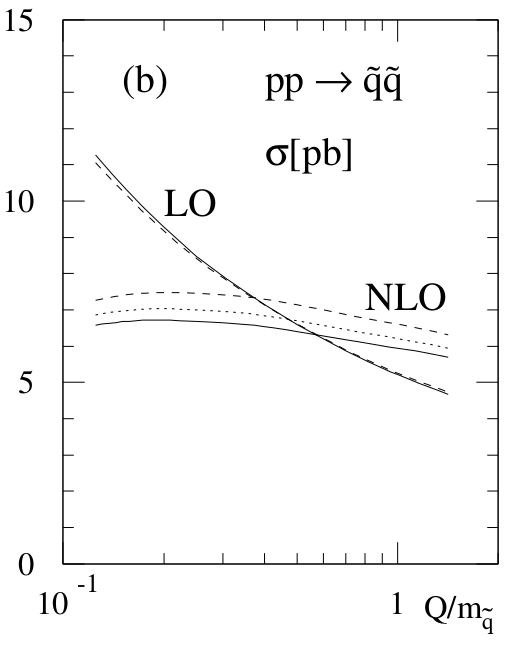
\includegraphics[scale=0.4]{squark_gluino_LO_NLO.png}
\caption{The dependence on the renormalization/factorization scale $Q$ for the LO and NLO cross sections for squark-squark production at the LHC ($\sqrt{s}=14$ TeV). Parton densities are GRV94 (solid), CTEQ3 (dashed) and MRS(A') (dotted). Mass parameters are $m_{\tilde{q}}=600$ GeV, $m_{\tilde{g}}=500$ GeV and $m_t=175$ GeV. Figure from \cite{beenakker1997squark}.}
\label{Fig:: hadron susy : LO vs NLO beenakker}
\end{figure}


The calculations from \cite{beenakker1997squark} assume degenerate squark masses $m_{\tilde{q}}$, set the 5 lightest quark masses to zero as they are much lighter than the squarks, and the top quark mass to $m_t =175$ GeV. The two free parameters left are then $m_{\tilde{g}}$ and $m_{\tilde{q}}$. This indicates that these might be good features for the learning. The renormalization scheme used is the $\bar{MS}$ scheme. Masses and couplings are renormalized, and the resulting parameters can be found in \cite{beenakker1997squark}.

\subsubsection{Nest-to-leading Order Partonic Cross-Section}

As previously discussed, calculations for hadron colliders require first finding the hadronic cross sections. In order to analyze these, scaling functions are introduced \cite{beenakker1997squark} giving the LO+NLO result as
\begin{align}
\hat{\sigma}_{ij} = \frac{\alpha_s^2(Q^2)}{m^2} \Big\{ &f^B_{ij}(\eta, r) + 4 \pi \alpha_s (Q^2) \Bigg[ f_{ij}^{V+S}(\eta, r, r_t) \nonumber \\ & + f_{ij}^H (\eta, r) + \bar{f}_{ij} (\eta, r) \log \Bigg( \frac{Q^2}{m^2}\Bigg) \Bigg] \Big\}
,
\end{align}
where $Q^2$ is the renormalization scale, often set to $Q^2 = m^2$, and $m = (\sqrt{p_1^2} + \sqrt{p_2^2})/2$ is the average mass of the produced particles. The scaling functions $f$ are as follows: the Born term $f^B$ from Eq.~(\ref{Eq:: susy hadron : Born term sigma}), the sum of virtual and soft-gluon corrections $f^{V+S}$, the hard gluon corrections $f^H$, and the scale-dependent contributions $\bar{f}$. The partonic cross section depends on the parameters
\begin{align}
&\eta = \frac{s}{4m^2} -1, &r= \frac{m_{\tilde{g}}^2}{m_{\tilde{q}}^2}, &&r_t = \frac{m_t^2}{m^2}.
\end{align}


\subsubsection{Hadronic Cross-Section}

As per the above discussion, the partonic cross-sections must be integrated over in order to obtain the total hadronic cross section. A convolution integral over the parton distribution functions yields the expression 
\begin{align}
\sigma(S, Q^2) = \sum_{i,j=q, q, \bar{q}} \int_{\tau}^1dx_1 \int_{\tau/x_1}^1 dx_2 f_i^{h_1} (x_1, Q^2) f_j^{h_2}(x_2, Q^2) \hat{\sigma}_{ij} (x_1x_2S, Q^2)\Big|_{\tau=4m^2/S}.
\end{align}
The integrals are calculated numerically using the VEGAS integration routine \cite{PETERLEPAGE1978192} in \cite{beenakker1997squark}.
The uncertainty due to different parameterizations of the parton densities for the LHC calculations of the NLO terms amount to $\lesssim 13 \%$ at the central scale.

\subsubsection{K-Factor}

To quantify the change in the cross section found by adding NLO terms, the \textit{$K$-factor} is introduced. The $K$-factor is the ratio between the cross sections
\begin{align}
K = \sigma_{NLO}/\sigma_{LO}.
\end{align}
The $K$-factor for squark production for varying mass ratios $m_{\tilde{q}}/m_{\tilde{g}}=2.0$, $ 1.6$, $1.2$, $0.8$ at the LHC is shown in Fig.\ \ref{Fig:: susy hadron : K-factor LHC}. As seen from the figure, the $K$-factor is larger than one and quite stable as a function of the squark mass. 

\begin{figure}
\centering
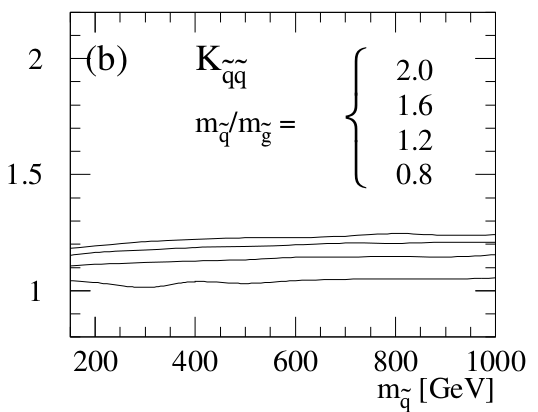
\includegraphics[scale=0.5]{squark_gluino_K_factor.png}
\caption{The $K$-factors for the LHC ($\sqrt{s}=14$ TeV). Parton densities are GRV94, with scale $Q=m$, and the top squark mass is $m_t=175$ GeV. Figure from \cite{beenakker1997squark}.}
\label{Fig:: susy hadron : K-factor LHC}
\end{figure}


\subsection{State-of-the-art Tools}

There are two numerical tools for the calculation of NLO SUSY cross sections, namely Prospino \cite{beenakker1996prospino} and NLL-fast \cite{beenakker2016nlo+}.

\subsubsection{Prospino}\label{Sec:: susy hadron : Prospino}
\verb|Prospino 2.1| \cite{beenakker1996prospino} is a numerical tool that calculates supersymmetric cross sections to next-to-leading order for non-degenerate squark masses. It uses the $K$-factor to calculate NLO cross sections, by first computing LO cross sections for the 5 or 4 lightest squark flavors. The LO and NLO rates are then calculated for a mean value of the squark mass, and the corresponding $K$-factor is calculated. The LO cross sections for different squarks are then multiplied by the $K$-factor, giving an approximation to the NLO terms for non-degenerate masses. The calculations are outlined in the section above, and are described in more detail in \cite{beenakker1996prospino}. 

\verb|Prospino 2.1| is quite time-consuming, however. Evaluating the strong process cross sections for just a single CMSSM benchmark point takes about 15 minutes of CPU time on a modern processor \cite{balazs2017colliderbit}. 

In addition, as was discovered during the project, \verb|Prospino 2.1| has a weakness in the heavy squark mass space. Consider the cross section for the production of $\tilde{c}_L \tilde{c}_L$. When all squark masses are heavy, but $m_{\tilde{c}_L}$ is slightly lighter than the others, the $K$-factor can be set to zero if the average mass is above threshold ($\tau > s$). This means that $LO \neq 0$ and $NLO =0$, which gives problematic outlier points that cause trouble during learning.



\subsubsection{NLL-fast}

\verb|NLL-fast 2.1| \cite{beenakker1997squark, kulesza2009threshold, kulesza2009soft, beenakker2009soft, beenakker2011squark} computes the hadronic cross sections of gluino and squark pair production including NLO supersymmetric QCD corrections, and the resummation of soft gluon emission at next-to-leading-logarithmic (NLL) accuracy. It also provides an error estimation, based on the errors from renormalization scale dependence and the parton distribution functions. The calculation is done by reading in tables of LO and NLO+NLL results, the scale uncertainty and the PDF and $\alpha_s$ error, and uses fast interpolation to calculate cross sections for any squark and gluino mass within the range $[200, 2500]$ GeV for $\sqrt{s}=8$ TeV. This does mean, however, that \verb|NLL-fast 2.1| is limited in that it only calculates cross sections for mass-degenerate squarks. Since the true total cross section for squark pair production consists of 36 different cross sections for combinations of the 4 lightest quarks, the estimate from \verb|NLL-fast 2.1| is very simplified and unfit for \textit{e.g.} MSSM-24, as shown in a later section.

\subsubsection{Accuracy}

Including the NLO+NLL cross sections has reduced the theoretical error to $10 \%$ for a wide range of processes and masses, see the discussion in \cite{balazs2017colliderbit}. There are other uncertainties, however, such as the ones from the PDFs and $\alpha_s$. These must also be included in the total error estimate. PDFs are based on experimental data, and so the uncertainty increases with the sparticle masses because the PDFs are most poorly constrained at large scales and at large partons $x$.

To illustrate, consider both the gluino and (degenerate) squark mass to be $1.5$ TeV, which is at the edge of what the LHC is able to produce at 8 TeV, as mentioned in the above section. \verb|NLL-fast 2.1| gives errors of $(+24.3 \%, -22.2\%)$ for the PDFs and $(+8.3 \%, -7.3 \%)$ for $\alpha_s$, when using the MSTW2008 NLO PDF
set \cite{Martin:2009iq}. In this case the total error will not be much lower than $25 \%$. However, with new data from the LHC errors from PDFs and $\alpha_s$ will be reduced over time.

Thus, the relative regression errors obtained in this thesis should not exceed $10 \%$, in order to keep the regression errors subdominent.




\bibliographystyle{plain}
\bibliography{dingsen_susy_at_hadron_colliders}

\end{document}
